\begin{figure}[p]
\centering
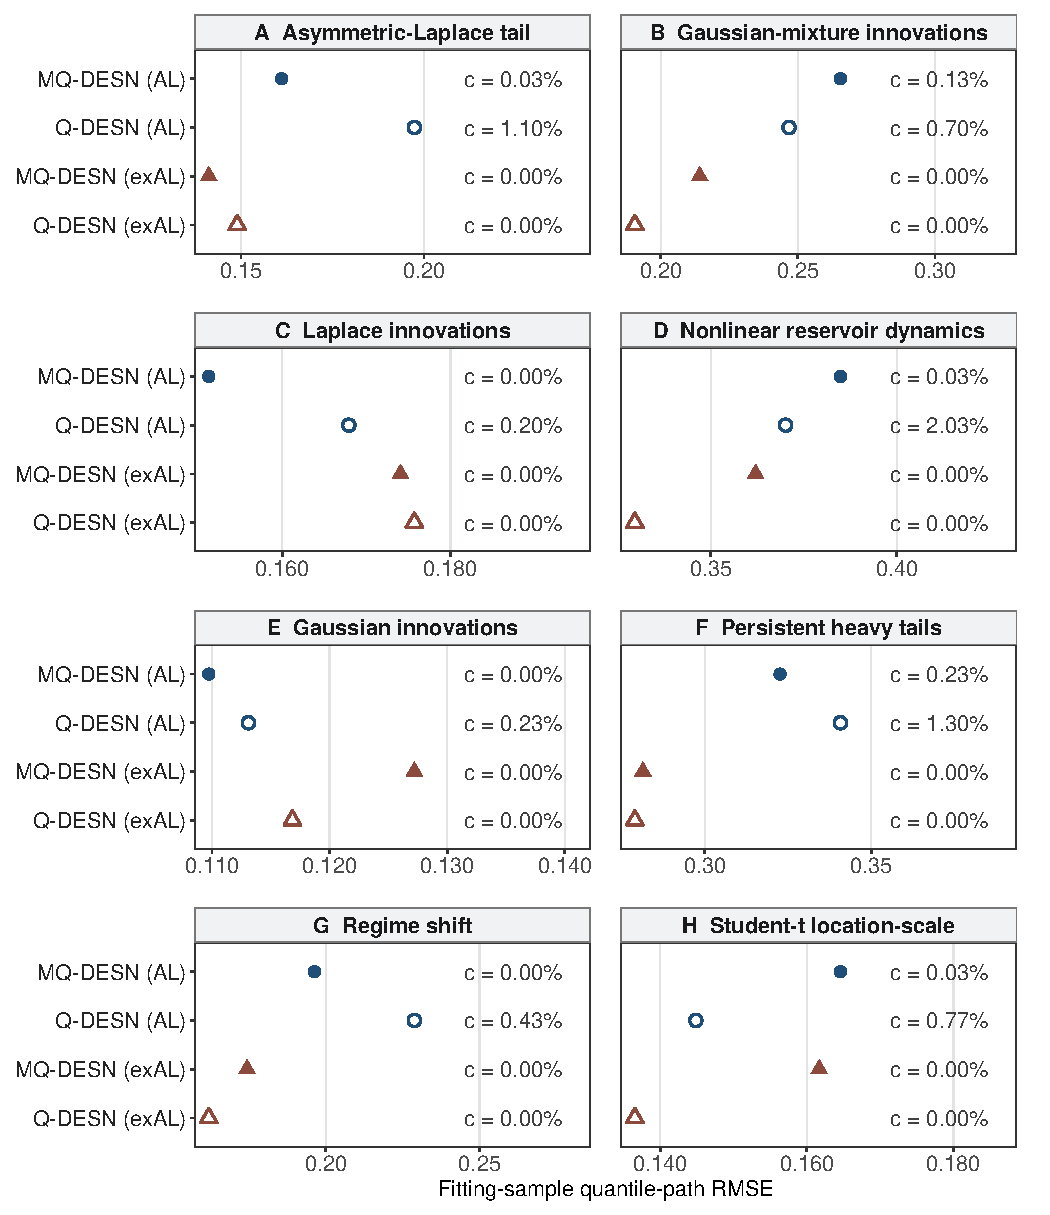
\includegraphics[width=0.94\textwidth]{figures/joint_qdesn_simulation/joint_qdesn_pure_desn_v2_mq_fit_oracle_rmse.pdf}
\caption{Fitting-sample recovery of known conditional quantile paths in the multiquantile study. Points give the RMSE of monotone posterior-mean grids, not posterior interval summaries. Annotations \(c\) give raw adjacent-level crossing percentages before projection. Q--DESN fits levels independently; MQ--DESN estimates their coefficients jointly.}
\label{fig:joint-qdesn-pure-desn-v2-fit-rmse}
\end{figure}
